\subsection{\RxRx}\label{sec:app_rxrx1}

High-throughput screening techniques that can generate large amounts of data
are now common in many fields of biology,
including transcriptomics~\citep{harrill2019tox},
genomics~\citep{echeverri2006high,zhou2014high}, proteomics and
metabolomics~\citep{taylor2021spatially}, and drug
discovery~\citep{broach1996high, macarron2011impact, swinney2011were,
boutros2015microscopy}.
Such large volumes of data, however, need to be created in experimental batches, or groups of experiments executed at similar times under similar conditions.
Despite attempts to carefully control experimental variables such as
temperature, humidity, and reagent concentration, measurements from
these screens are confounded by technical artifacts that arise from differences
in the execution of each batch.
These \emph{batch effects} make it difficult to draw conclusions from data  across experimental batches~\citep{leek2010tackling,parker2012practical,soneson2014batch,nygaard2016methods,caicedo2017data}.

We study the shift induced by batch effects on a variant of the \RxRx
dataset~\citep{taylor2019rxrx1}.
As illustrated in \reffig{dataset_rxrx1}, there are significant visual
differences between experimental batches, making recognizing siRNA perturbations
in OOD experiments in the \RxRx dataset a particularly challenging task for
existing ML algorithms.

\subsubsection{Setup}\label{sec:app_rxrx1_setup}

\paragraph{Problem setting.}
We consider the domain generalization setting, where the domains are
experimental batches and we seek to generalize to images from unseen experimental
batches. Concretely, the input $x$ is a 3-channel image of cells obtained by
fluorescent microscopy, the label $y$ indicates which of the 1,139 genetic
treatments (including no treatment) the cells received, and the domain $d$
specifies the experimental batch of the image.

\paragraph{Data.}
\RxRx was created by Recursion (recursion.com) in its automated high-throughput
screening laboratory in Salt Lake City, Utah. It is comprised of fluorescent microscopy images of
human cells in four different cell lines: HUVEC, RPE, HepG2, and U2OS.  These
were acquired via fluorescent microscopy using a 6-channel variant of the
\emph{Cell Painting} assay~\citep{bray2016cell}.
\reffig{rxrx1_channels} shows an example of the cellular contents of each of
these 6 channels: nuclei, endoplasmic reticuli, actin, nucleoli and cytoplasmic
RNA, mitochondria, and Golgi.
To make the dataset smaller and more accessible, we only included the first 3 channels in \RxRx.
\begin{figure}[t]
    \centering
    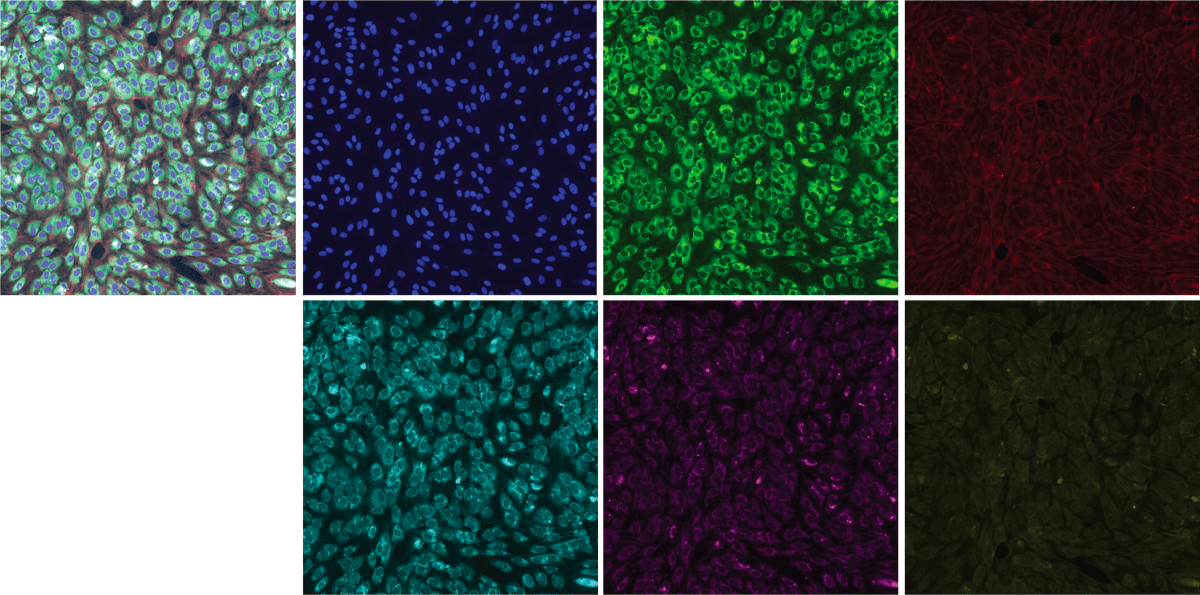
\includegraphics[width=0.9\linewidth]{figures/rxrx1_channels.png}
    \caption{6-channel composite image of HUVEC cells (left) and its
      individual channels (rest): nuclei (blue), endoplasmic reticuli (green),
      actin (red), nucleoli and cytoplasmic RNA (cyan), mitochondria (magenta),
      and Golgi (yellow). The overlap in channel content is due in part to the
      lack of complete spectral separation between fluorescent stains. Note that
      only the first 3 channels are included in \RxRx.}
    \label{fig:rxrx1_channels}
\end{figure}

The images in \RxRx are the result of executing the same experimental
design 51 different times, each in a different batch of experiments. The design
consists of four 384-well plates, where individual wells are used to isolate
populations of cells on each plate (see \reffig{rxrx1_plate}).
\begin{figure}[t]
    \centering
    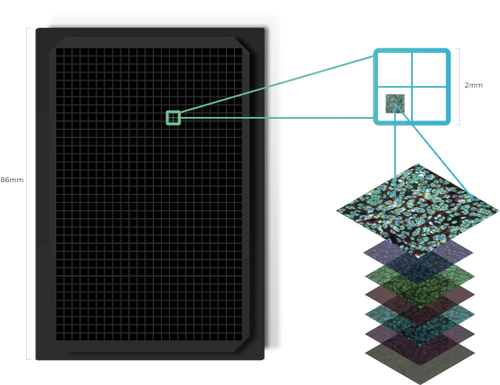
\includegraphics[width=0.5\linewidth]{figures/rxrx1_plate.png}
    \caption{Schematic of a 384-well plate demonstrating imaging sites and
      6-channel images. The 4-plate experiments in \RxRx were run in the wells
      of such 384-well plates. \RxRx contains two imaging sites per well.}
    \label{fig:rxrx1_plate}
\end{figure}
The wells are laid out in a 16$\times$24 grid, but only the wells in the inner
14$\times$22 grid are used since the outer wells are most susceptible to
environmental factors. Of these 308 usable wells, one is left untreated to
provide a \emph{negative control} phenotype, while the rest are treated with
small interfering ribonucleic acid, or siRNA, at a fixed concentration. Each
siRNA is designed to knockdown a single target gene via the RNA interference
pathway, reducing the expression of the gene and its associated
protein~\citep{tuschl2001rna}. However, siRNAs are known to have significant but
consistent off-target effects via the microRNA pathway, creating partial
knockdown of many other genes as well. The overall effect of siRNA transfection
is to perturb the morphology, count, and distribution of cells, creating a
\emph{phenotype} associated with each siRNA. The phenotype is sometimes visually
recognizable, but often the effects are subtle and hard to detect.

In each plate, 30 wells are set aside for 30 \emph{positive control} siRNAs. Each has a different gene as its primary target, which together with the
single untreated well already mentioned, provides a set of reference phenotypes
per plate. Each of the remaining 1,108 wells of the design (277 wells~$\times$~4
plates) receives one of 1,108 \emph{treatment} siRNA, respectively, so that
there is at most one well of each treatment siRNA in each experiment. We say
at most once because, although rare, it happens that either an siRNA is not
correctly transferred into the designated destination well, resulting in an
additional untreated well, or an operational error is detected by quality
control procedures that render the well unsuitable for inclusion in the dataset.

Each experiment was run in a single cell type, and of the 51 experiments in \RxRx, 24 are in HUVEC, 11 in RPE, 11 in HepG2, and 5 in U2OS.
\reffig{rxrx1_celltypes} shows the phenotype of the same siRNA in each of these
four cell types.
\begin{figure}[tbp]
    \centering
    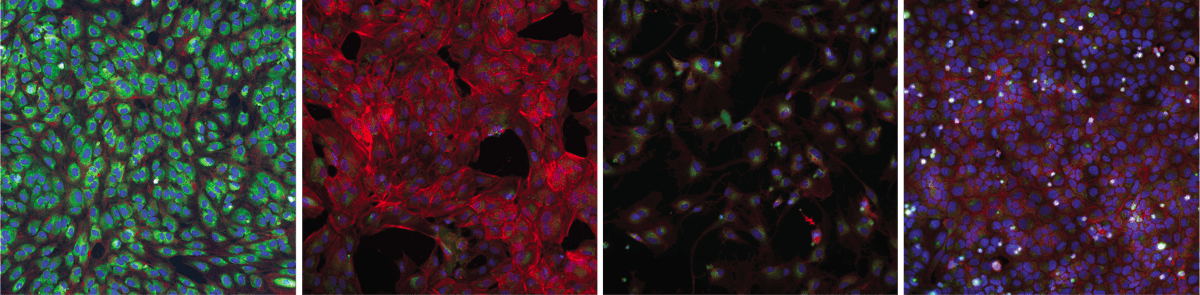
\includegraphics[width=0.9\linewidth]{figures/rxrx1_celltypes.png}
    \caption{Images of the same siRNA in four cell types, from left to right: HUVEC, RPE, HepG2, U2OS.}
    \label{fig:rxrx1_celltypes}
\end{figure}

We split the dataset by experimental batches, with the training and test splits having roughly the same composition of cell types:
\begin{enumerate}
  \item \textbf{Training:} 33 experiments (16 HUVEC, 7 RPE, 7 HepG2, 3 U2OS),
    site 1 only = 40,612 images.
  \item \textbf{Validation (OOD):} 4 experiments (1 HUVEC, 1 RPE, 1 HepG2, 3
    U2OS), sites 1 and 2 = 9,854 images.
  \item \textbf{Test (OOD):} 14 experiments (7 HUVEC, 3 RPE, 3 HepG2, 1
    U2OS), sites 1 and 2 = 34,432 images.
  \item \textbf{Test (ID):} same 33 experiments as in the training set, site 2
  only = 40,612 images.
\end{enumerate}
In addition to the class (siRNA), each image is associated with the following
metadata: cell type, experiment, plate, well, and site.
We emphasize that all the images of an experiment are found in exactly one of
the training, validation (OOD) or test (OOD) splits. See
\refapp{app_rxrx1_details} for more data processing details.

\paragraph{Evaluation.}
We evaluate models by their average accuracy across test images. Note that there
are two images per well in the test set, which we evaluate independently.

The cell types are not balanced in the training and test sets.
Correspondingly, we observed higher performance on the HUVEC cell type, which is over-represented, and lower performance on the U2OS cell type, which is under-represented.
While maintaining high performance on minority (or even unseen) cell types is an important problem, for \RxRx, we opt to measure the average accuracy across all experiments instead of, for example, the worst accuracy across cell types.
This is because the relatively small amount of training data available from the minority cell type (U2OS) makes it challenging to cast \RxRx as a tractable subpopulation shift problem.
We also note that the difference in performance across cell types leads to the validation performance being significantly lower than the test performance, as there is a comparatively smaller fraction of HUVEC and a comparatively higher fraction of U2OS.

\paragraph{Potential leverage.}
By design, there is usually one sample per class per experiment in the training
set, with the following exceptions: 1) there are usually four samples per
positive control, though 2) samples may be missing, as described above.
Moreover, while batch effects can manifest themselves in many complicated ways,
it is the case that the training set consists of a large number of experiments
selected randomly amongst all experiments in the dataset, hence we
expect models to be able to learn what is common amongst all such samples per
cell type, and for that ability to generalize to to test batches. We emphasize
that, whether in the training or test sets, the same cell types are perturbed
with the same siRNA, and thus the phenotypic distributions for each batch share
much of the same generative process.

We also note that, while not exploited here, there is quite a bit of structure
in the \RxRx dataset. For example, except in the case of errors, all treatment
siRNA appear once in each experiment, and all control conditions appear once per
plate, so four times per experiment. Also, due to the operational efficiencies
gained, the 1,108 treatment siRNAs always appear in the same four groups of 277
per experiment.  So while the particular well an siRNA appears in is randomized,
it will always appear with the same group of 276 other siRNAs. This structure
can be exploited for improving predictive accuracy via post-prediction methods
such as linear sum assignment. However, such methods do not represent improved
generalization to OOD samples, and should be avoided.

\subsubsection{Baseline results}

\paragraph{Model.} For all experiments, we train the standard ResNet-50 model
\citep{he2016resnet} pretrained on ImageNet, using a learning rate of $1e-4$ and
$L_2$-regularization strength of $1e-5$. We trained these models with the Adam
optimizer, using default parameter values $\beta_{1} = 0.9$ and $\beta_{2} =
0.999$, with a batch size of 75 for 90 epochs, linearly increasing the learning
rate for 10 epochs, then decreasing it following a cosine learning rate schedule.
We selected hyperparameters by a grid search over learning rates $\{10^{-5}$, $10^{-4}$, $10^{-3}\}$, $L_2$-regularization strengths $\{10^{-5}, 10^{-3}\}$,
and numbers of warmup epochs $\{5, 10\}$.
We report results aggregated over 3 random seeds.

\paragraph{ERM results and performance drops.}
Model performance dropped significantly going from the train-to-train in-distribution (ID) setting to
the official out-of-distribution (OOD) setting (\reftab{results_rxrx1}),
with an average accuracy of 35.9\% on the ID test set but only 29.9\% on the OOD test set for ERM.
\begin{table*}[t!]
  \caption{Baseline results on \RxRx. In-distribution (ID) results correspond to the train-to-train setting. Parentheses show standard deviation across
  3 replicates.}
  \label{tab:results_rxrx1}
  \centering
  \begin{tabular}{lcccc}
  \toprule
  Algorithm & Validation (OOD) accuracy & Test (ID) accuracy & Test (OOD) accuracy\\
  \midrule
  ERM       & 19.4 (0.2) & 35.9 (0.4) & \textbf{29.9} (0.4) \\
  CORAL     & 18.5 (0.4) & 34.0 (0.3) & 28.4 (0.3) \\
  IRM       & 5.6 (0.4) & 9.9 (1.4) & 8.2 (1.1) \\
  Group DRO & 15.2 (0.1) & 28.1 (0.3) & 23.0 (0.3) \\
  \bottomrule
  \end{tabular}
\end{table*}

\begin{table*}[!t]
  \caption{Mixed-to-test comparison for ERM models on \RxRx.
  In the official OOD setting, we train on data from 33 experiments (1 site per experiment) and test on 14 different experiments (2 sites per experiment).
  In the mixed-to-test setting, we replace 14 of the training experiments with 1 site from each of the test experiments, which keeps the training set size the same, but halves the test set size.
  Parentheses show standard deviation across 3 replicates.
  }
  \label{tab:drop_rxrx1}
  \centering
  \begin{tabular}{lcccc}
  \toprule
  Setting & Algorithm & Test (OOD) accuracy\\
  \midrule
  Official      (train on ID examples)         & ERM & 29.9 (0.4)\\
  Mixed-to-test (train on ID + OOD examples)   & ERM & \textbf{39.8} (0.2) \\
  \bottomrule
  \end{tabular}
\end{table*}

We ran an additional mixed-to-test comparison, where we moved half of the OOD test set into the training set, while keeping the overall amount of training data the same.
Specifically, we moved one site per experiment from the OOD test set into the training set, and discarded an equivalent number of training sites, while leaving the validation set unchanged.
While the test set in the mixed-to-test setting is effectively half as large as in the standard split, we expect it to be distributed similarly, since the two test set versions comprise the same 14 experiments.

\reftab{drop_rxrx1} shows that there is a large gap between the OOD test accuracies in the official setting (29.9\%) and the test accuracies in the mixed-to-test setting (39.8\%).
We note that the latter is higher than the train-to-train ID test accuracy of 35.9\% reported in \reftab{results_rxrx1}.
This difference mainly stems from the slight difference in cell type composition between the test sets in the train-to-train and mixed-to-test settings; in particular, the train-to-train test set has a slightly higher proportion of the minority cell type (U2OS), on which performance is worse, and a slightly lower proportion of the majority cell type (HUVEC), on which performance is better.
In this sense, the mixed-to-test result of 39.8\% is a more accurate reflection of in-distribution performance on this dataset, and the results in \reftab{results_rxrx1} therefore understate the magnitude of the distribution shift.


\paragraph{Additional baseline methods.}
We also trained models with CORAL, IRM, and group DRO, treating each experiment
as a domain, and using the same model hyperparameters as ERM.
However, the models trained using these methods all performed poorly compared to the ERM model (\reftab{results_rxrx1}).
One complication with these methods is that the experiments in the training set comprise different cell types, as mentioned above; this heterogeneity can pose a challenge to methods that treat each domain equivalently.

\paragraph{Discussion.}
An important observation about batch effects in biological experiments: it is
often the case that batch effects are mediated via biological mechanisms. For
example, an increase in cellular media concentration may lead to cell growth and
proliferation, while the upregulation of proliferation genes will do the same.
Thus the ``nuisance'' factors associated with batch effects are often correlated
with the biological signal we are attempting to observe, and cannot be
disentangled from the biological factors that explain the data. Correction algorithms
should take account of such trade-offs and attempt to optimize for both
correction and signal preservation.

\subsubsection{Broader context}
As previously mentioned, high-throughput screening techniques are used broadly
across many areas of biology, and therefore batch effects are a common problem
in fields such as genomics, transcriptomics, proteomics, metabolomics, etc., so
a particular solution in one such area may prove to be applicable in many areas
of biology~\citep{goh2017batch}.

There are other datasets that are used in studying batch effects. The one most
comparable to \RxRx is the BBBC021 dataset~\citep{ljosa2012annotated}, which
contains 13,200 3-channel fluorescent microscopy images of MCF7 cells acquired
across 10 experimental batches. A subset of 103 treatments from 38 drug
compounds belonging to 12 known mechanism of action (MoA) groups was first
studied in~\cite{ando2017improving}, and has been the subject of subsequent
studies~\citep{caicedo2018weakly,godinez2018unsupervised,tabak2020correcting}.
Note that this dataset differs dramatically from RxRx1, in that there are fewer
images, treatments, batches, and cell types, and each batch contains only a
small subset of the total treatments.

\subsubsection{Additional details}\label{sec:app_rxrx1_details}
\paragraph{Data processing.}
\RxRx contains two non-overlapping 256$\times$256 fields of view per well.
Therefore, there could be as many as 125,664 images in the dataset (= 51 experiments~$\times$~4 plates/experiment~$\times$~308 wells/plate~$\times$~2 images/well).
154 images were removed based on data quality, leaving a total dataset of 125,510 images.

\paragraph{Modifications to the original dataset.} The underlying raw dataset
consists of 2048~$\times$~2048 pixel, 6 channel, 16bpp images. To fit within the
constraints of the \Wilds benchmark, images for \RxRx were first downsampled to
1024~$\times$~1024 and 8bpp, cropped to the center 256~$\times$~256 pixels, and only the
first three channels (nuclei, endoplasmic reticuli, actin) were retained. The
original RxRx1 dataset, available at rxrx.ai and described in \citet{taylor2019rxrx1}, provides 512~$\times$~512 center
crops of the downsampled images with all 6 channels retained.

The original RxRx1 dataset was also used in a NeurIPS 2019 competition hosted on Kaggle. The validation (OOD) and test (OOD) splits in \RxRx correspond to the public and private test sets from the Kaggle competition. The original RxRx1 dataset did not have an additional test (ID) split, and thus the original training split had both sites 1 and 2, for a total of 81,442 images.
The Kaggle competition also aggregated predictions from both sites to form a single prediction per well, whereas in \RxRx, we treat each site separately.

As described in \refsec{app_rxrx1_setup}, each plate in both the training and test sets contains the
same 31 control conditions (one untreated well, and 30 positive control siRNAs).
The Kaggle competition provided the labels for these control conditions in the test set, expecting that competitors would use them for various domain alignment techniques such as CORAL. However, these labels were instead used by the top competitors to bootstrap pseudo-labeling techniques.
For \RxRx, for consistency with the other datasets and the typical domain generalization setting, we have opted not to release these control test labels for training.

The poor performance reported here on \RxRx may seem
surprising in light of the fact that the top finishers of the Kaggle
competition achieved near perfect accuracy on the test (OOD) set. This difference is due to a number of factors, including:
\begin{enumerate}
  \item Adjustments made to the original RxRx1 dataset for \RxRx, as detailed in this subsection.
  \item Differences in the network architectures used. To make training on \RxRx more accessible, we used a less compute-intensive architecture than typical in the competition.
  \item Differences in training techniques used like pseudo-labeling (using the test control labels, as described above) and batch-level dataset augmentations or ensembling.
  \item Differences in the way accuracy is measured. In the Kaggle competition, accuracy was measured for each well, meaning site-level predictions were aggregated to well-level predictions, and only for treatment classes, whereas in \RxRx, for convenience, accuracy is measured at each site and for both treatment and control classes.
  \item The use of post-prediction methods like linear sum assignment that exploited the particular structure of the experiments in the RxRx1 dataset, as described under Potential Leverage in \refsec{app_rxrx1_setup}.
\end{enumerate}
